% Short data paper template
%% Created by Simon Hengchen and Nilo Pedrazzini for the Journal of Open Humanities Data (https://openhumanitiesdata.metajnl.com)


\documentclass{article}

\usepackage{algorithm}
\usepackage{algpseudocode}
\usepackage[english]{babel}
\usepackage[utf8]{inputenc}
\usepackage{johd}
\usepackage{amsmath}
\usepackage{tikz}
\usepackage{array}
\usepackage{graphicx} 
\usepackage{subcaption}
\usepackage{amssymb}
\usepackage{geometry}
\setlength{\parindent}{0pt}
\title{Federative Learning}
\usetikzlibrary{arrows.meta,decorations.pathreplacing,positioning}
\author{ \\
}
\date{}

\begin{document}
\maketitle

\section*{Problème}

On dispose de d'un ensemble $\mathcal{W}$ travailleurs de cardinal $W$. Parmi eux, on a les travailleurs réguliers $\mathcal R \subset \mathcal W$ de cardinal $R$. Et les travailleurs empoisonnés $\mathcal W \setminus \mathcal R$.


% --- PREMIER DESSIN : espace d'échantillonnage Ω et sous-ensemble W ---
\begin{center}
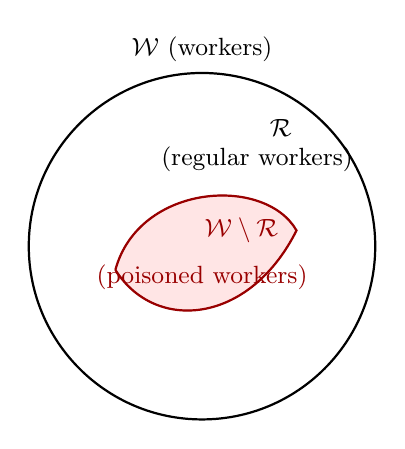
\begin{tikzpicture}[scale=1, every node/.style={font=\small}]
  % Grand disque (Omega)
  \draw[thick] (0,0) circle (2.2cm);
  \node at (0,2.5) {$\mathcal W$ (workers)};

  % Sous-ensemble W (portion interne)
  \begin{scope}
    \clip (0,0) circle (2.2cm);
    \fill[red!10, draw=red!60!black] (-1.1,-0.3) .. controls (-0.8,0.8) and (0.8,0.9) .. (1.2,0.2) .. controls (0.6,-1.0) and (-0.6,-1.1) .. (-1.1,-0.3);
    \draw[red!60!black, thick] (-1.1,-0.3) .. controls (-0.8,0.8) and (0.8,0.9) .. (1.2,0.2) .. controls (0.6,-1.0) and (-0.6,-1.1) .. (-1.1,-0.3);
  \end{scope}

  \node[red!60!black] at (0.5,0.2) {$\mathcal W \setminus \mathcal R$};
  \node[red!60!black] at (0,-0.4) {\small (poisoned workers)};

  \node at (1,1.5) {$\mathcal R$};
  \node at (0.7,1.1) {\small (regular workers)};
\end{tikzpicture}
\end{center}


Le nombre exact et l'identité
des travailleurs réguliers sont inconnus du serveur. L'objectif est de résoudre le problème
d'optimisation distribué suivant, défini uniquement sur les travailleurs réguliers :

\begin{equation}
    \min_{x \in \mathbb{R}^D} f(x)
    = \frac{1}{R} \sum_{w \in \mathcal{R}} f_w(x),
    \label{eq:global_cost}
\end{equation}

où la fonction de coût locale de chaque travailleur régulier $w \in \mathcal{R}$ est définie par :

\begin{equation}
    f_w(x) = \frac{1}{J} \sum_{j=1}^{J} f_{w,j}(x),
\end{equation}

chaque travailleur possédant $J$ échantillons.\\ 

De plus, les travailleurs empoisonnés de l'ensemble $\mathcal W \setminus \mathcal R$ disposent de données dont les étiquettes ont été corrompues mais, malgré ces erreurs, ils appliquent strictement le protocole algorithmique du système distribué.

\section*{Solution: Algorithme du moment stochastique distribué}

Le problème \eqref{eq:global_cost} est résolu à l'aide de l'algorithme du \emph{moment stochastique distribué}.

À chaque itération $t$, le serveur diffuse le modèle global $x_t$ à tous les travailleurs.  
Chaque travailleur $w$ sélectionne alors un échantillon $i_t^w$ uniformément dans $\{1,\dots,J\}$ et
calcule un gradient stochastique. \\

Pour un travailleur régulier $w \in \mathcal{R}$, la mise à jour du moment local est :

\begin{equation}
    m_t^{w} = (1 - \alpha) m_{t-1}^{w}
    + \alpha \nabla f_{w, i_t^w}(x_t),
\end{equation}

où $\alpha \in [0,1]$ est le coefficient inertiel.

Pour un travailleur empoisonné $w \in \mathcal{W} \setminus \mathcal{R}$, la mise à jour correspondante est :

\begin{equation}
    \tilde{m}_t^{w} = (1 - \alpha) \tilde{m}_{t-1}^{w}
    + \alpha \nabla \tilde{f}_{w, i_t^w}(x_t),
\end{equation}

où $\tilde{f}_{w,j}$ désigne une fonction de coût utilisant une étiquette falsifiée.

Nous notons de manière unifiée le message envoyé au serveur :

\begin{equation}
    \hat{m}_t^{w} =
    \begin{cases}
        m_t^{w}, & \text{si } w \in \mathcal{R}, \\
        \tilde{m}_t^{w}, & \text{si } w \in \mathcal{W} \setminus \mathcal{R}.
    \end{cases}
\end{equation}

Le serveur reçoit l'ensemble des messages $\{\hat{m}_t^{w}\}_{w \in \mathcal{W}}$ et applique un agrégateur, $\mathrm{Agg}$,
(robuste ou non) pour calculer la mise à jour globale du modèle via une étape de descente:


\begin{equation}
    x^{t+1} = x^t - \gamma \cdot \mathrm{Agg}(\{\hat{m}_w^t : w \in \mathcal{W}\}),
    \label{eq:update_robust}
\end{equation}

\begin{algorithm}[h]
\caption{Moment stochastique distribué}
\label{alg:momentum}
\begin{algorithmic}[1]
\State \textbf{Entrée :} Initialisations $x^0 \in \mathbb{R}^D$,
$m_{w}^{-1} = \nabla f_{w,i_0^w}(x^0)$ si $w \in \mathcal{R}$,
$\tilde{m}_{w}^{-1} = \nabla \tilde{f}_{w,i_0^w}(x_0^w)$ si $w \in \mathcal{W} \setminus \mathcal{R}$ ;  
l'indice initial $i_0^w$ tiré uniformément dans $\{1,\dots,J\}$ ;  
pas d’apprentissage $\gamma$ ; coefficient inertiel $\alpha$ ;  
nombre total d’itérations $T$.

\For{$t = 0, 1, \dots, T-1$}
    \State Le serveur diffuse $x^t$ à tous les travailleurs.
    \State Travailleur régulier $w \in \mathcal{R}$ :
    \State \hspace{0.8cm} Tire uniformément $i_t^w \in \{1,\dots,J\}$.
    \State \hspace{0.8cm} Met à jour $m_w^t = (1 - \alpha) m_w^{t-1} + \alpha \nabla f_{w,i_t^w}(x^t)$.
    \State \hspace{0.8cm} Envoie $m_w^t$ au serveur.
    \State Travailleur empoisonné $w \in \mathcal{W}\setminus\mathcal{R}$ :
    \State \hspace{0.8cm} Tire uniformément $i_t^w \in \{1,\dots,J\}$.
    \State \hspace{0.8cm} Met à jour $\tilde{m}_w^t = (1 - \alpha)\tilde{m}_w^{t-1} + \alpha \nabla \tilde{f}_{w,i_t^w}(x^t)$.
    \State \hspace{0.8cm} Envoie $\tilde{m}_w^t$ au serveur.
    \State Le serveur reçoit $\{\hat{m}_w^t : w \in \mathcal{W}\}$ et met à jour $x^{t+1}$ selon \eqref{eq:update_robust}.
\EndFor
\end{algorithmic}
\end{algorithm}

\section{Postulat de l'article}


\section*{Etude des hypothèses}

\paragraph{Assumption 3}

$\forall x \in \mathbb R^D,\,\displaystyle \max_{w \in \mathcal R} \|\nabla f_w(x) - \nabla f(x)\| \leq \xi$

% --- DEUXIEME DESSIN : deux boules concentriques (petite + grande) et vecteurs gradient ---
\begin{center}
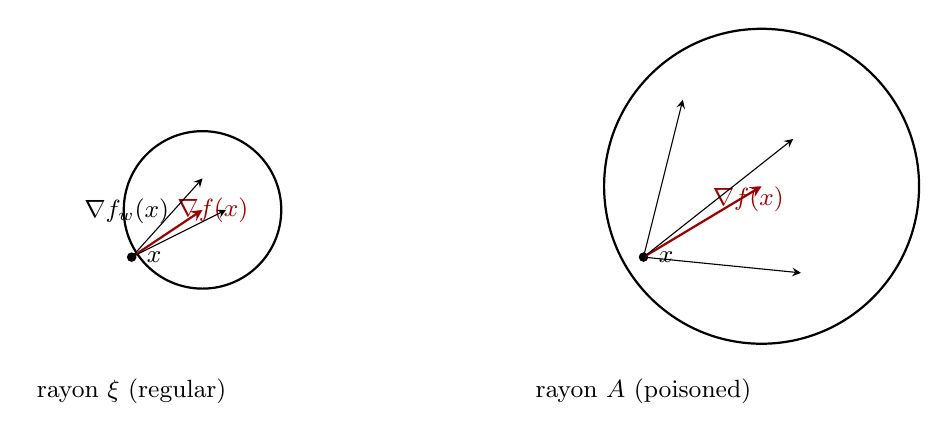
\begin{tikzpicture}[scale=1, every node/.style={font=\small}]
  % Petite boule (à gauche)
  \begin{scope}[xshift=-4.5cm]
    \draw[thick] (0.9,0.6) circle (1cm) node[above,yshift=6mm] {\small \textbf{}};
    \node at (0,-1.7) {\small rayon $\xi$ (regular)};

    % Centre x
    \filldraw[black] (0,0) circle (1.5pt) node[right=2pt] {$x$};

    % vecteurs (petit rayon)
    \draw[red!60!black, thick][->,>=stealth] (0,0) -- (0.9,0.6) node[midway, above right] {\small $\nabla f(x)$};
    \draw[->,>=stealth] (0,0) -- (1.2,0.6) node[midway, above left] {\small $\nabla f_w(x)$};
    \draw[->,>=stealth] (0,0) -- (0.9,1);
  \end{scope}

  % Grande boule (à droite)
  \begin{scope}[xshift=2.0cm]
    \draw[thick] (1.5,0.9) circle (2.cm) node[above,yshift=8mm] {\small \textbf{}};
    \node at (0,-1.7) {\small rayon $A$ (poisoned)};

    % Centre x
    \filldraw[black] (0,0) circle (1.5pt) node[right=2pt] {$x$};

    % vecteurs (plus longs pour illustrer)
    \draw[red!60!black, thick][->,>=stealth] (0,0) -- (1.5,0.9) node[midway, above right] {\small $\nabla f(x)$};
    \draw[->,>=stealth] (0,0) -- (1.9,1.5) node[midway, below right] {\small $\ $};
    \draw[->,>=stealth] (0,0) -- (0.5,2);
    \draw[->,>=stealth] (0,0) -- (2,-0.2);
  \end{scope}
\end{tikzpicture}
\end{center}

\section{Robust Aggregator}

Pour $y_1,...,y_W \in R^D$, et $\bar y = \dfrac{1}{R}\displaystyle\sum_{w\in \mathcal R} y_w$,

$$\|Ragg(\{y_1,...,y_W\} - \bar y\| \leq \rho \cdot \max_{w \in \mathcal R}\|y_w - \bar y\|$$

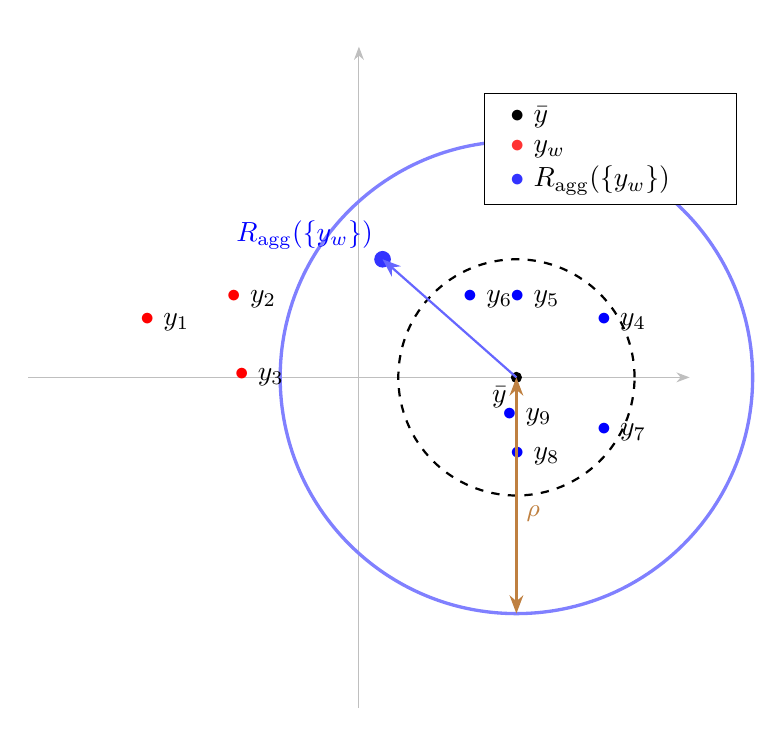
\begin{tikzpicture}[>=Stealth, scale=1.0]

  % parameters (you can change these)
  \def\rmax{1.5}     % radius corresponding to max_w ||y_w - \bar y||
% rho factor (for the smaller circle)
  \def\npoints{7}     % number of points y_w to draw

  % center (bar y)
  \coordinate (b) at (2,0);
  \coordinate (p) at (-1, 0);

  % draw axes (optional)
  \draw[->,gray!50] (-4.2,0) -- (4.2,0) node[right] {};
  \draw[->,gray!50] (0,-4.2) -- (0,4.2) node[above] {};

  % draw circle of max radius
  \draw[dashed, thick] (b) circle[radius=\rmax];
  \node[gray] at ({\rmax+0.4}, -0.25) {};

  % draw smaller rho-circle
  \draw[blue!50, very thick] (b) circle[radius={2*\rmax}];
  \node[blue] at (0.45, 0.6) {};
  \node[right] at (-2.9,0.7) {\textcolor{red}{$\bullet$} $y_1$};
  \node[right] at (-1.8,1) {\textcolor{red}{$\bullet$} $y_2$};
  \node[right] at (-1.7,0) {\textcolor{red}{$\bullet$} $y_3$};

  \node[right] at (2.9,0.7) {\textcolor{blue}{$\bullet$} $y_4$};
  \node[right] at (1.8,1) {\textcolor{blue}{$\bullet$} $y_5$};
  \node[right] at (1.2,1) {\textcolor{blue}{$\bullet$} $y_6$};
  \node[right] at (2.9,-0.7) {\textcolor{blue}{$\bullet$} $y_7$};
  \node[right] at (1.8,-1) {\textcolor{blue}{$\bullet$} $y_8$};
  \node[right] at (1.7,-0.5) {\textcolor{blue}{$\bullet$} $y_9$};

  % draw the center / mean
  \filldraw[black] (b) circle(1.8pt);
  \node[below left] at (b) {$\bar y$};

  % place y_w points around (on the large circle, slightly perturbed)
  
  % An example R_agg result (somewhere inside rho-circle)
  \coordinate (Ragg) at (0.3, 1.5);
  \filldraw[blue!80] (Ragg) circle(2.8pt) ;
  \node[above left, blue] at (Ragg) {$R_{\mathrm{agg}}(\{y_w \})$};

  % arrow showing the distance from bar y to Ragg
  \draw[->,blue!60,thick] (b) -- (Ragg) node[midway, right,font=\small] {};

  \draw[<->,brown,thick] (b) -- (2,-3) node[midway, below right,font=\small] {$\rho$};

  % bracket and equation annotation at bottom


  % legend box
  \begin{scope}[shift={(3.2,2.6)}]
    \draw[fill=white] (-1.6,-0.4) rectangle (1.6,1.0);
    \node[right] at (-1.4,0.7) {\textcolor{black}{$\bullet$} $\bar y$};
    \node[right] at (-1.4,0.3) {\textcolor{red!80}{$\bullet$} $y_w$ };
    \node[right] at (-1.4,-0.1) {\textcolor{blue!80}{$\bullet$} $R_{\mathrm{agg}}(\{y_w\})$};
  \end{scope}

\end{tikzpicture}


\section*{Théorèmes}

\paragraph{Théorème 17} : Avec un $\rho-\mathrm{RAgg}$, sous les hypothèses 2,3 et 4, pour $T\rightarrow \infty$,

$$\dfrac{1}{T}\sum_{t=1}^T \mathbb E\|\nabla f\|^2 \leq 15 \rho^2\xi^2 + O\left(\dfrac{1}{\sqrt{T}}\right)$$

\paragraph{Théorème 18} : Avec le mean-aggregator, sous les hypothèses 2,3,4 et 5, pour $T\rightarrow \infty$,

$$\dfrac{1}{T}\sum_{t=1}^T \mathbb E\|\nabla f\|^2 \leq 15 \delta^2 A^2 + O\left(\dfrac{1}{\sqrt{T}}\right)$$

Ainsi, lorsque $A\delta > \rho \xi$, on ne peut pas parler d'une supériorité de la moyenne.


\section*{Travail réalisé}

Pour vérifier empiriquement les résultats théoriques de l'article, nous avons mis en œuvre une simulation de l'environnement d'apprentissage fédéré décrit. Notre travail s'est articulé autour de plusieurs axes principaux : la configuration de l'environnement, l'implémentation de l'algorithme et des agrégateurs, et enfin la conduite d'expériences pour comparer leurs performances.

\paragraph{1. Environnement de Simulation}
Nous avons simulé un réseau d'apprentissage fédéré composé de $W$ travailleurs, en portant une attention particulière à la configuration des données, du modèle et du scénario d'attaque.

\subparagraph{a) Analyse et Distribution des Données}
Notre étude s'est appuyée sur trois jeux de données de référence pour la classification d'images : \textbf{MNIST}, \textbf{Fashion-MNIST} et \textbf{CIFAR-10}. Pour chacun, nous avons mené une analyse exploratoire à l'aide d'un script de visualisation dédié (`visualisation_data.py`). Cette analyse préliminaire nous a permis de :
\begin{itemize}
    \item \textbf{Visualiser des échantillons} d'images pour chaque jeu de données afin de vérifier leur intégrité et comprendre leur nature (chiffres manuscrits, articles de mode, objets variés).
    \item \textbf{Analyser la distribution des classes} via des histogrammes. Nous avons confirmé que ces trois jeux de données sont bien équilibrés, chaque classe étant représentée par un nombre d'exemples similaire, ce qui constitue une base saine pour l'entraînement.
    \item \textbf{Projeter l'espace des données} en 2D en utilisant une réduction de dimensionnalité (PCA puis t-SNE). Cette visualisation nous a donné un aperçu de la séparabilité intrinsèque des classes pour chaque jeu de données.
\end{itemize}
Pour les simulations d'apprentissage fédéré, l'ensemble d'entraînement de chaque jeu de données a été distribué entre les $W$ travailleurs de manière \textbf{IID (Indépendante et Identiquement Distribuée)}. Concrètement, les données ont été mélangées aléatoirement, puis partitionnées en $W$ sous-ensembles de taille égale. Chaque travailleur dispose ainsi d'un jeu de données local qui est statistiquement représentatif de la distribution globale.

\subparagraph{b) Modèles d'Apprentissage}
Nous avons implémenté trois modèles distincts en PyTorch, de complexité croissante, afin d'évaluer la robustesse de l'approche sur différentes architectures :
\begin{itemize}
    \item \textbf{Régression Logistique (`LogisticRegression`)} : Un modèle linéaire simple, sans couche cachée, prenant en entrée une image vectorisée. Il sert de baseline pour isoler l'impact des attaques dans un cadre simple.
    \item \textbf{Perceptron Multi-Couches (`MLP`)} : Un réseau de neurones dense avec une ou plusieurs couches cachées et des fonctions d'activation non-linéaires (e.g., ReLU). Ce modèle offre une capacité de représentation supérieure à la régression logistique.
    \item \textbf{Réseau de Neurones Convolutif (`CNN`)} : Une architecture plus complexe utilisant des couches de convolution et de pooling, particulièrement adaptée au traitement d'images. Ce modèle est conçu pour extraire des caractéristiques spatiales et atteindre de meilleures performances sur des tâches comme CIFAR-10.
\end{itemize}
Pour chaque modèle, la sortie est une couche linéaire à 10 neurones (un par classe), et la fonction de coût `CrossEntropyLoss` de PyTorch est utilisée, appliquant implicitement une fonction Softmax.

\subparagraph{c) Scénarios d'Attaque par Empoisonnement}
Nous avons modélisé une attaque par empoisonnement des données (\textit{data poisoning}), où une fraction $\delta = (W-R)/W$ des travailleurs est malveillante. Ces travailleurs, dits "empoisonnés", cherchent à dégrader les performances du modèle global.
\begin{itemize}
    \item \textbf{Inversion d'étiquette (`label_flipping`)} : Il s'agit d'une attaque ciblée où les étiquettes d'une classe source sont systématiquement remplacées par celles d'une classe cible. Par exemple, pour MNIST, nous avons configuré cette attaque pour changer toutes les étiquettes `3` en `7`. L'objectif est de forcer le modèle à mal classifier une classe spécifique.
    \item \textbf{Inversion d'étiquette aléatoire (`label_shuffling`)} : Dans cette variante non ciblée, les étiquettes de l'ensemble des données d'un travailleur empoisonné sont mélangées de manière aléatoire. Chaque image se voit ainsi attribuer une étiquette incorrecte (avec une forte probabilité), ce qui vise à dégrader la performance globale du modèle plutôt qu'à cibler une classe particulière.
    \item \textbf{Attaque par ajout de bruit (`noise_attack`)} : Cette attaque n'altère pas les étiquettes mais corrompt les données d'entrée elles-mêmes. Un bruit significatif (par exemple, un bruit Gaussien) est ajouté aux pixels des images des travailleurs empoisonnés. L'objectif est d'injecter des données de mauvaise qualité qui vont perturber l'apprentissage des features pertinentes par le modèle.
    \item \textbf{Comportement de l'attaquant :} Il est crucial de noter que les travailleurs empoisonnés, bien que disposant de données corrompues, suivent par ailleurs scrupuleusement le protocole de communication défini par l'algorithme \ref{alg:momentum}. Ils calculent et envoient leurs mises à jour de moment comme n'importe quel travailleur régulier, rendant leur détection non triviale pour le serveur central.
\end{itemize}

\paragraph{2. Implémentation de l'Algorithme}
Nous avons implémenté l'algorithme du moment stochastique distribué (Algorithm \ref{alg:momentum}) en Python, en nous appuyant sur la bibliothèque PyTorch pour la gestion des modèles et le calcul des gradients. Notre implémentation distingue clairement le rôle du serveur et celui des travailleurs, en intégrant la capacité de simuler des comportements malveillants complexes.
\begin{itemize}
    \item \textbf{Serveur :} Le serveur orchestre le processus d'apprentissage. À chaque itération $t$, il effectue les actions suivantes :
    \begin{enumerate}
        \item Il diffuse les poids du modèle global actuel, $x^t$, à l'ensemble des $W$ travailleurs.
        \item Il collecte les vecteurs de moment calculés $\{\hat{m}_w^t\}_{w \in \mathcal{W}}$ de chaque travailleur.
        \item Il applique une règle d'agrégation (Moyenne ou Médiane) sur les vecteurs reçus pour obtenir un moment agrégé $m_{\text{agg}}^t = \mathrm{Agg}(\{\hat{m}_w^t\})$.
        \item Il met à jour le modèle global en effectuant une étape de descente de gradient : $x^{t+1} = x^t - \gamma \cdot m_{\text{agg}}^t$.
    \end{enumerate}

    \item \textbf{Travailleurs :} Chaque travailleur, qu'il soit régulier ou malveillant, exécute un cycle de calcul local.
    \begin{enumerate}
        \item Il reçoit le modèle global $x^t$ du serveur.
        \item Il sélectionne un mini-batch de données depuis son jeu de données local.
        \item Il calcule le gradient stochastique $\nabla f_{w, i_t^w}(x^t)$ sur ce batch en utilisant la fonction de coût `CrossEntropyLoss`.
        \item Il met à jour son vecteur de moment local : $m_w^t = (1 - \alpha) m_w^{t-1} + \alpha \nabla f_{w,i_t^w}(x^t)$.
        \item Il renvoie son moment mis à jour, $\hat{m}_w^t$, au serveur.
    \end{enumerate}

    \item \textbf{Comportement des Travailleurs Malveillants :} La distinction cruciale réside dans la manière dont les travailleurs malveillants génèrent leur message $\hat{m}_w^t$. Notre implémentation, inspirée par `label_poisoning.py`, permet de simuler deux grandes familles d'attaques :
    \begin{itemize}
        \item \textbf{Attaques par empoisonnement des données :} Pour les attaques de type `label_flipping`, `backdoor_poisoning`, etc., le travailleur malveillant suit exactement le protocole ci-dessus, mais sur un jeu de données local préalablement corrompu. Le gradient calculé, $\nabla \tilde{f}_{w,i_t^w}(x^t)$, est donc intrinsèquement biaisé, ce qui empoisonne le moment $m_w^t$ qui est ensuite envoyé.
        \item \textbf{Attaques sur les gradients (`sign_flip_attack`, `scale_attack`)} : Dans ce scénario plus direct, le travailleur malveillant peut d'abord calculer un gradient honnête $\nabla f_{w,i_t^w}(x^t)$ (ou un autre vecteur), puis le manipuler \textit{explicitement} avant de l'envoyer. Par exemple, avec `sign_flip_attack`, il envoie $\hat{m}_w^t = -\text{sign}(\nabla f_{w,i_t^w}(x^t))$. Cette approche ne correspond pas directement à l'algorithme \ref{alg:momentum} (qui suppose un empoisonnement des données), mais représente une menace byzantine plus puissante que nous avons également étudiée.
    \end{itemize}
\end{itemize}

\paragraph{3. Agrégateurs}
Le point central de notre étude était de comparer l'agrégateur de moyenne standard à plusieurs agrégateurs robustes implémentés dans le fichier `aggregators.py`. Ces derniers sont conçus pour mitiger l'impact des mises à jour malveillantes envoyées par les travailleurs empoisonnés.
\begin{itemize}
    \item \textbf{Moyenne (`agg_mean`)} : Il s'agit de l'agrégateur de référence qui calcule simplement la moyenne arithmétique des vecteurs de moment reçus. Bien qu'efficace en l'absence d'attaque, il est extrêmement vulnérable : un seul vecteur malveillant avec des valeurs arbitrairement grandes peut corrompre totalement la moyenne.
    
    \item \textbf{Moyenne Élégauée (`agg_trimmed_mean`)} : Pour chaque coordonnée, cette méthode trie les valeurs de tous les travailleurs, écarte une fraction (`trim_ratio`) des plus petites et des plus grandes valeurs, puis calcule la moyenne sur les valeurs restantes. Elle est robuste tant que la proportion d'attaquants est inférieure à `trim_ratio`.
    
    \item \textbf{Médiane Coordonnée par Coordonnée (`agg_coord_median`)} : C'est un exemple typique d'agrégateur robuste. Pour chaque coordonnée (c'est-à-dire pour chaque paramètre du modèle), il calcule la \textit{médiane} des valeurs provenant de tous les travailleurs. La médiane étant insensible aux valeurs extrêmes (jusqu'à 50\% d'attaquants), cet agrégateur peut ignorer les contributions malveillantes.
    
    \item \textbf{Écrêtage Centré (`agg_centered_clipping`)} : Cette méthode calcule d'abord la moyenne des vecteurs. Ensuite, pour chaque vecteur, elle calcule sa différence par rapport à la moyenne. Si la norme de cette différence dépasse un seuil (`clip_threshold`), le vecteur de différence est réduit pour correspondre à ce seuil. Enfin, la moyenne des vecteurs ainsi ajustés est retournée.
    
    \item \textbf{FABA (`agg_faba_simple`)} : Cette approche itérative vise à filtrer les attaquants. À chaque étape, elle calcule la moyenne des vecteurs restants et supprime celui qui en est le plus éloigné (en norme euclidienne). Ce processus est répété un certain nombre de fois (défini par `remove_frac`), puis la moyenne des vecteurs restants est calculée.
    
    \item \textbf{LFighter (`agg_lfighter_simple`)} : Cette méthode utilise un algorithme de clustering (KMeans) pour partitionner les vecteurs de mise à jour en `n_clusters` groupes. Elle part du principe que les travailleurs honnêtes formeront le plus grand cluster. L'agrégateur identifie ce cluster majoritaire et calcule la moyenne des seuls vecteurs qui en font partie, ignorant ainsi les autres clusters potentiellement malveillants.
\end{itemize}

\paragraph{4. Expériences et Analyse}
Nous avons mené une série d'expériences pour évaluer l'impact de l'attaque par empoisonnement et l'efficacité de l'agrégateur robuste.
\begin{itemize}
    \item \textbf{Scénarios :} Les simulations ont été exécutées avec différents pourcentages de travailleurs empoisonnés (par exemple, 10\%, 30\%, 40\%).
    \item \textbf{Métriques :} Nous avons suivi l'évolution de la précision du modèle global sur un jeu de test non corrompu, ainsi que la fonction de coût globale au fil des itérations d'entraînement.
    \item \textbf{Résultats observés :} Les résultats expérimentaux ont montré que, en présence d'un nombre significatif de travailleurs empoisonnés, les performances du modèle s'effondrent rapidement lorsque l'agrégateur est la moyenne. En revanche, l'utilisation de la médiane coordonnée par coordonnée a permis de maintenir une précision élevée, mitigant efficacement l'impact de l'attaque. Ces observations valident l'intuition des théorèmes 17 et 18 : lorsque l'attaque est suffisamment forte ($A\delta$ grand), un agrégateur robuste (avec un $\rho$ borné) offre une bien meilleure garantie de performance.
\end{itemize}

En conclusion, notre travail pratique a permis de reproduire les conditions d'une attaque par empoisonnement de données en apprentissage fédéré et de démontrer expérimentalement la supériorité d'un agrégateur robuste par rapport à la moyenne, conformément aux prédictions théoriques de l'article.


\end{document}